%
% File - ch1.tex
%
%
% Description:
% This file should contain the first real chapter or section of your
% thesis.
%
%
%%%%%%%%%%%%%%%%%%%%%%%%%%%%%%%%%%%%%%%%%%%%%%%%%%%%%%%%%%%%%%%%%%%%%%%%%%%%%%%
\section{Quadtree Background}~\label{sec:quadtree_motivation}
%%%%%%%%%%%%%%%%%%%%%%%%%%%%%%%%%%%%%%%%%%%%%%%%%%%%%%%%%%%%%%%%%%%%%%%%%%%%%%%

A quadtree is a tree data structure that designates each internal node
to have exactly 4 children. Quadtrees are used to partition a 2D space
by recursively subdividing it into 4 quadrants or regions. The regions
may be square or rectangular or may have arbitrary shapes. Quadtrees
may be classified according to the type of data represented such as
areas, points, lines and curves. Figure~\ref{fig:quadtree}
demonstrates a set of 2D data points that have been used to compose a
quadtree. The reasoning for using a quadtree structure is that any
region search that requires the data points within a polygon area
simply can reference the tree rather than the data.  There are clear
search benefits from the data to tree representations. In the case of
the lower right quadrant, any region search will consult the tree
structure and determine that only a limited number of point values 
(X, Y) are required for comparison.  In short, the tree representation
saves the computational calculations for the polygon search by
immediately directing that only a limited number of points exist in
that entire quadrant.  In the comparison case, it is easier for a
polygon that resides in the lower right quadrant to consult the tree
versus consult the full data set using full brute force checking of
every datapoint within the polygon range.

\begin{figure} [H]
    \begin{center}
    \vspace{0.5in}
    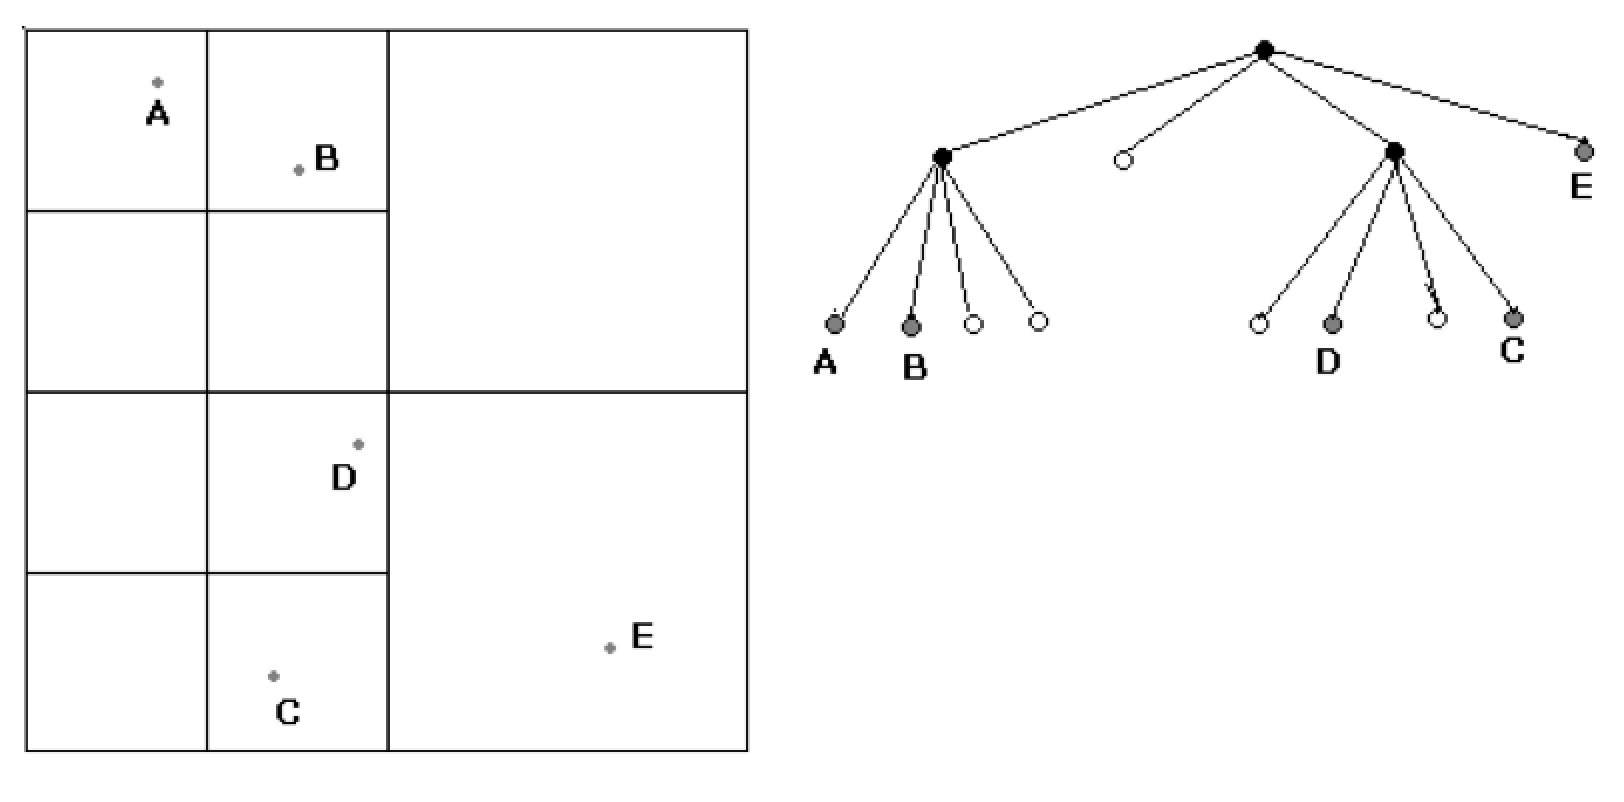
\includegraphics[scale=0.5]{Images/webQuad}
    \vspace{0.5in}
    \end{center}
    \caption{Example of Data Points Mapped within a Quadtree Data Structure.}
    \label{fig:quadtree}
\end{figure}



\subsection{Quadtree Construction}

Figure~\ref{fig:quadtree_construction1},
Figure~\ref{fig:quadtree_construction2},
Figure~\ref{fig:quadtree_construction3},
Figure~\ref{fig:quadtree_construction4}, demonstrates quadtree
construction on the CPU up to level 4.
The Figure~\ref{fig:quadtree_construction1}, shows the sample data points
at level 1 and it represents the root node containing all the data points.
The Figure~\ref{fig:quadtree_construction2}, shows the sample data points
at level 2 and it represents the four child nodes of the root node.
The Figure~\ref{fig:quadtree_construction2} is further subdivided to generate 
level 3 of the quadtree as shown in Figure~\ref{fig:quadtree_construction3}.
The Figure~\ref{fig:quadtree_construction4}, represents the tree at level 4.
There are two empty nodes at level 4, as there no points in that direction. 

 \begin{figure}[H]   
 \centering
 \vspace{0.5in}
 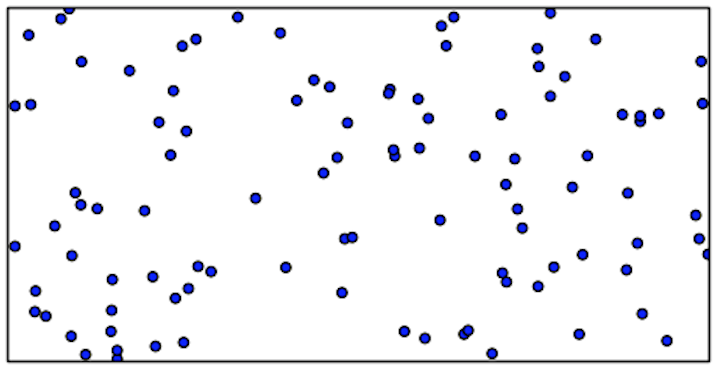
\includegraphics[scale=0.5]{Images/Quadtree_construction1}
 \vspace{0.5in}
 \caption{Level 1 of Quadtree.}
 \label{fig:quadtree_construction1}
 \end{figure}


 \begin{figure}[H]
 \centering
 \vspace{0.5in}
 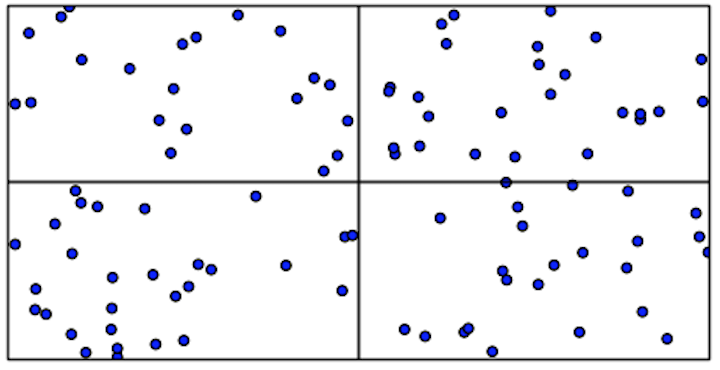
\includegraphics[scale=0.5]{Images/Quadtree_construction2}
 \vspace{0.5in}
 \caption{Level 2 of Quadtree.}
 \label{fig:quadtree_construction2}
 \end{figure}  

  \begin{figure}[H]    
  \centering
  \vspace{0.5in}
  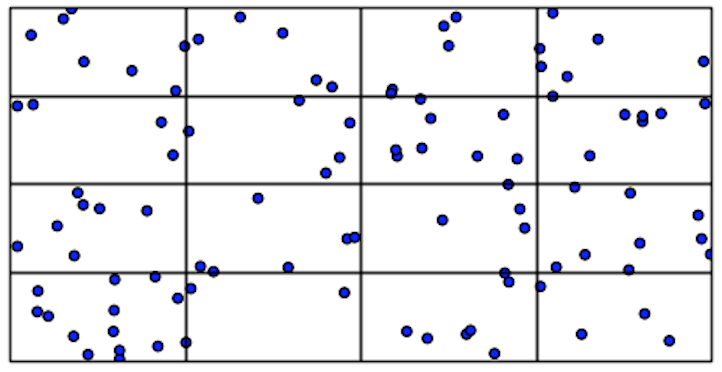
\includegraphics[scale=0.5]{Images/Quadtree_construction3}
  \vspace{0.5in}
  \caption{Level 3 of Quadtree.}
  \label{fig:quadtree_construction3} 
  \end{figure}

 \begin{figure}[H]    
 \centering
 \vspace{0.5in}
 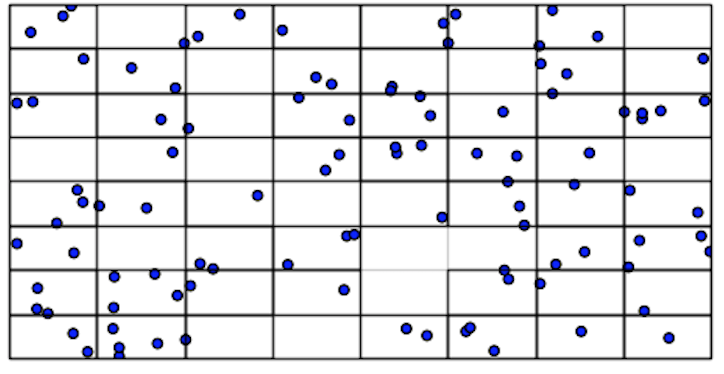
\includegraphics[scale=0.5]{Images/Quadtree_construction4}
 \vspace{0.5in}
 \caption{Level 4 of Quadtree.}
 \label{fig:quadtree_construction4}
 \end{figure}


The point quadtree structure recursively divides space into four equal 
rectangles based on the location of the points. The root of the quadtree 
represents the whole 2D space. Successive points divide each 
new sub-region into quadrants until all points are indexed. With each 
subsequent level, quadtrees can have a maximum of four children for 
every parent node. Each node represents a region in the 2D space
which contains a subset of the data points.

The common algorithm to construct a quadtree is based on sequential
 point insertion and this sequential approach is not suitable for
 massively parallel processors. Therefore the quadtree construction is
 done on the CPU. The performance of quadtrees, for Insertion is O(n
 log n), for searching is O(log n) and optimization for the purposes
 of balancing the tree is O(n log n) \cite{Kelly:gpu}. This makes quadtrees an ideal data
 structure for multiple insertion of points and range searching \cite{Kelly:gpu}.
 Though the linear quadtrees reduce the overhead involved in
 transferring the tree from the CPU main memory to the GPU memory, the
 pointer based quadtree has several other advantages. The pointer
 based quadtrees are more memory space efficient and it can be accessed
 in any traversal order by following the pointers whereas the linear
 quadtrees only allow preorder traversal and require logarithm time
 searches to find the next child for any other order~\cite{shaff:quad}.
 
The quadtree is built using pointers.
The tree is built by recursive function calls and sequentially inserting 
the points. Each parent node has pointers to all of its children. 
There are 3 structures in the quadtree, the node, the point and the 
point buffers.

Each node is one of three types which are the root node, link node and the leaf
node. The root node, corresponds to the entire array of input
points. The four children of the root node represent the 4 quadrants 
(Northwest - NW, Northeast - NE, Southwest - SW, Southeast - SE). The
link node is a node that can be further subdivided and the leaf nodes
correspond to the quadrants for which further subdivision is not
necessary.

The point structure is the input points to the quadtree which occupies
a 2D space. A leaf node has a list of point buffers, each of which
holds predetermined maximum number of points. Starting at the root, 
the quadrant or the direction (NW, NE, SW or SE) in which the input point 
lies is determined and a child node is built in that direction. 
This step is 
repeated till the leaf node is reached. 

The Figure~\ref{fig:Childquad}
shows the node index and its corresponding direction on its parent node. 
 Then the point is added to that leaf
node's buffer of points. If the buffer exceeds some predetermined
maximum number of elements, the points are moved into the next buffer
in the buffer list. The root node is subdivided recursively. The
quadtree with k levels including the root would have ${(4(k-1))}$
nodes on the k\textsuperscript{th} level and ((4k) $-1$) nodes in total~\cite{Kelly:gpu}.

 \begin{figure}[H]    
 \centering
 \vspace{0.5in}
 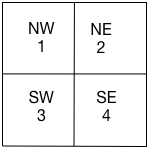
\includegraphics[scale=0.8]{Images/Childquad}
 \vspace{0.5in}
 \caption{NW - North west, NE - North east, SW - South west and SE - South east.}
 \label{fig:Childquad}
 \end{figure}

%%%%%%%%%%%%%%%%%%%%%%%%%%%%%%%%%%%%%%%%%%%%%%%%%%%%%%%%%%%%%%%%%%%%%%%%%%%%%%%
\section{Related Work}~\label{sec:relatedWork}
%%%%%%%%%%%%%%%%%%%%%%%%%%%%%%%%%%%%%%%%%%%%%%%%%%%%%%%%%%%%%%%%%%%%%%%%%%%%%%%

Traversal path for each polygon may differ, therefore linearizing the tree based on the traversal path for each polygon and iterating over the linear traversal order is computationally intensive.
Several application-specific approaches have been proposed to handle the problem.
 In algorithms like Barnes-Hut,  a point's traversal can be computed without executing the entire algorithm and a preprocessing pass can determine each point's linear traversal, avoiding repeatedly visiting interior nodes during vector operations. However, for PIP search, where a point's full traversal is only determined as the traversal progresses, the preprocessing step can be expensive.
 
Goldfarb et al. [2015]~\cite{goldfarb13sc} demonstrates a GPU implementation of tree traversal algorithms by installing ropes, extra pointers that connect a node in the tree not to its children,  instead to the next new node that a point would visit if its children are not visited. But the drawback of using ropes is that it requires an additional traversal prior to performing the actual traversals to create the ropes into the nodes of the tree structure. As a result, earlier attempts to use ropes to accelerate tree traversals have relied on application-specific transformations that leverage the semantics of the algorithm to efficiently place ropes.
The problem with using "Autoropes"~\cite{goldfarb13sc} is that since the rope pointers are computed during traversal and they are stored on the stack, it causes overhead due to stack manipulation and the efficiency is compromised.

Work by Zhang et al. [2013]~\cite{DBLP:journals/gis/ZhangY13} presents a speed up of 90x by constructing a quadtree using parallel primitives by transforming a multidimensional geospatial computing problem into chaining a set of generic parallel primitives that are designed for one dimensional arrays.

Another work by Bedorf et al. [2015]~\cite{Bedorf:2012:SOG:2133856.2134140} presents an octree construction where the tree is constructed on the GPU after mapping particles in 3D space to linear array. And a vectorized BFS traversal is done on the octree.

All of these implementations have relied on linearizing the tree for BFS traversal on the GPU or they have preprocessed the tree to either linearize or install extra pointers on the tree. 
CUDA GPU ray traversal through a hierarchical data structure such as a bounding volume hierarchy (BVH) is usually carried out using depth-first search by maintaining a stack.
This paper explores the parallelization of breadth-first search (BFS) to implement range search on GPUs. The kernel is optimized to minimize thread divergence and memory access. BFS is used instead of depth-first search (DFS) as it is easier to parallelize and implement efficiently on the GPU. BFS and DFS are fundamental building blocks for more sophisticated algorithms used in many computational fields that range from gaming, image processing to social network analysis. BFS is  used as a core computational kernel in a number of benchmark suites, including Rodinia, Parboil and the Graph500 supercomputer benchmark.

%%%%%%%%%%%%%%%%%%%%%%%%%%%%%%%%%%%%%%%%%%%%%%%%%%%%%%%%%%%%%%%%%%%%%%%%%%%%%%%
\section{Graphics Processing Unit Architecture}~\label{sec:gpu_overview}
%%%%%%%%%%%%%%%%%%%%%%%%%%%%%%%%%%%%%%%%%%%%%%%%%%%%%%%%%%%%%%%%%%%%%%%%%%%%%%%
%%%%%%%% GPU Hardware:
%DAC: GPU don't have cache, they are designed to exploit arithmetic intensity (high ratio of the number of arithmetic operations to the number of memory accesses).  Number of cores on a typical machine.  Use of shared memory has 1 cycle access and high-bandwidth for 16 threads per streaming multiprocessor).

The underlying architecture of the GPU is optimized for data-level
parallelism.  Taking a closer look at the
NVIDIA\textsuperscript{\textregistered} GPU reveals the chip is
organized into an array of highly threaded streaming multiprocessors 
(SMs). Each streaming multiprocessor consists of several streaming
processors (SPs). Streaming multiprocessors are grouped into thread
processing clusters (TPCs). The number of SPs per SM depends on the
generation of the chip.  

%TODO: Add GPU FLOPS vs CPU FLOPS chart?
NVIDIA\textsuperscript{\textregistered} has chips that increase the
number of streaming processors (SP) from 240 to 2048. Each SP has a
multiply-add unit plus an additional multiply unit.  The combined
power of that many SPs in this GPU exceeds one
teraflop~\cite{Kirk:2010:PMP:1841511}.  Each SM contains a special function
unit which can compute floating-point functions such as square root
and transcendental functions.  Each streaming processor is threaded and
can run thousands of threads per application.  Graphics cards are
commonly built to run 5,000-12,000 threads simultaneously on this GPU.
The GTX680 can support 192 threads per SMX and a total of 1536 threads
 simultaneously~\cite{nvidia:12:gtx680tech}. In contrast, the
Intel\textsuperscript{\textregistered} Core\texttrademark i7 series
can support two threads per core.

GPUs are optimized via the execution throughput of a massive number of threads.
The hardware takes advantages of this by switching to different threads while 
other threads wait for long-latency memory accesses.  This methodology enables
very minimal control logic for each execution thread~\cite{Kirk:2010:PMP:1841511}.
Each thread is very lightweight and requires very little creation overhead.

From a memory perspective, the GPU is architected quite differently
than a CPU.  Each GPU currently comes with up to four gigabytes of
Graphics Double Data Rate (GDDR) DRAM which is used as global
memory. The GPU architecture is designed to exploit arithmetic
intensity and data-level parallelism.

Figure~\ref{fig:KeplerArch} shows the architecture of the GTX680.
This generation of the CUDA enabled GPU devices consists of an array of 8 
next generation streaming multiprocessors (SMX), 4 GPCs and 4 memory controllers.
Each GPC has a dedicated raster engine and two SMX units.
Figure~\ref{fig:gpu_architecture} shows the architecture of a SMX. 
Each SMX unit contains 192 cores and four warp schedulers. 
Each warp scheduler is capable of dispatching two instructions per warp every clock~\cite{nvidia:12:gtx680tech}.

%  GPU picture
\begin{figure} [H]
    \centering
    \vspace{0.5in}
    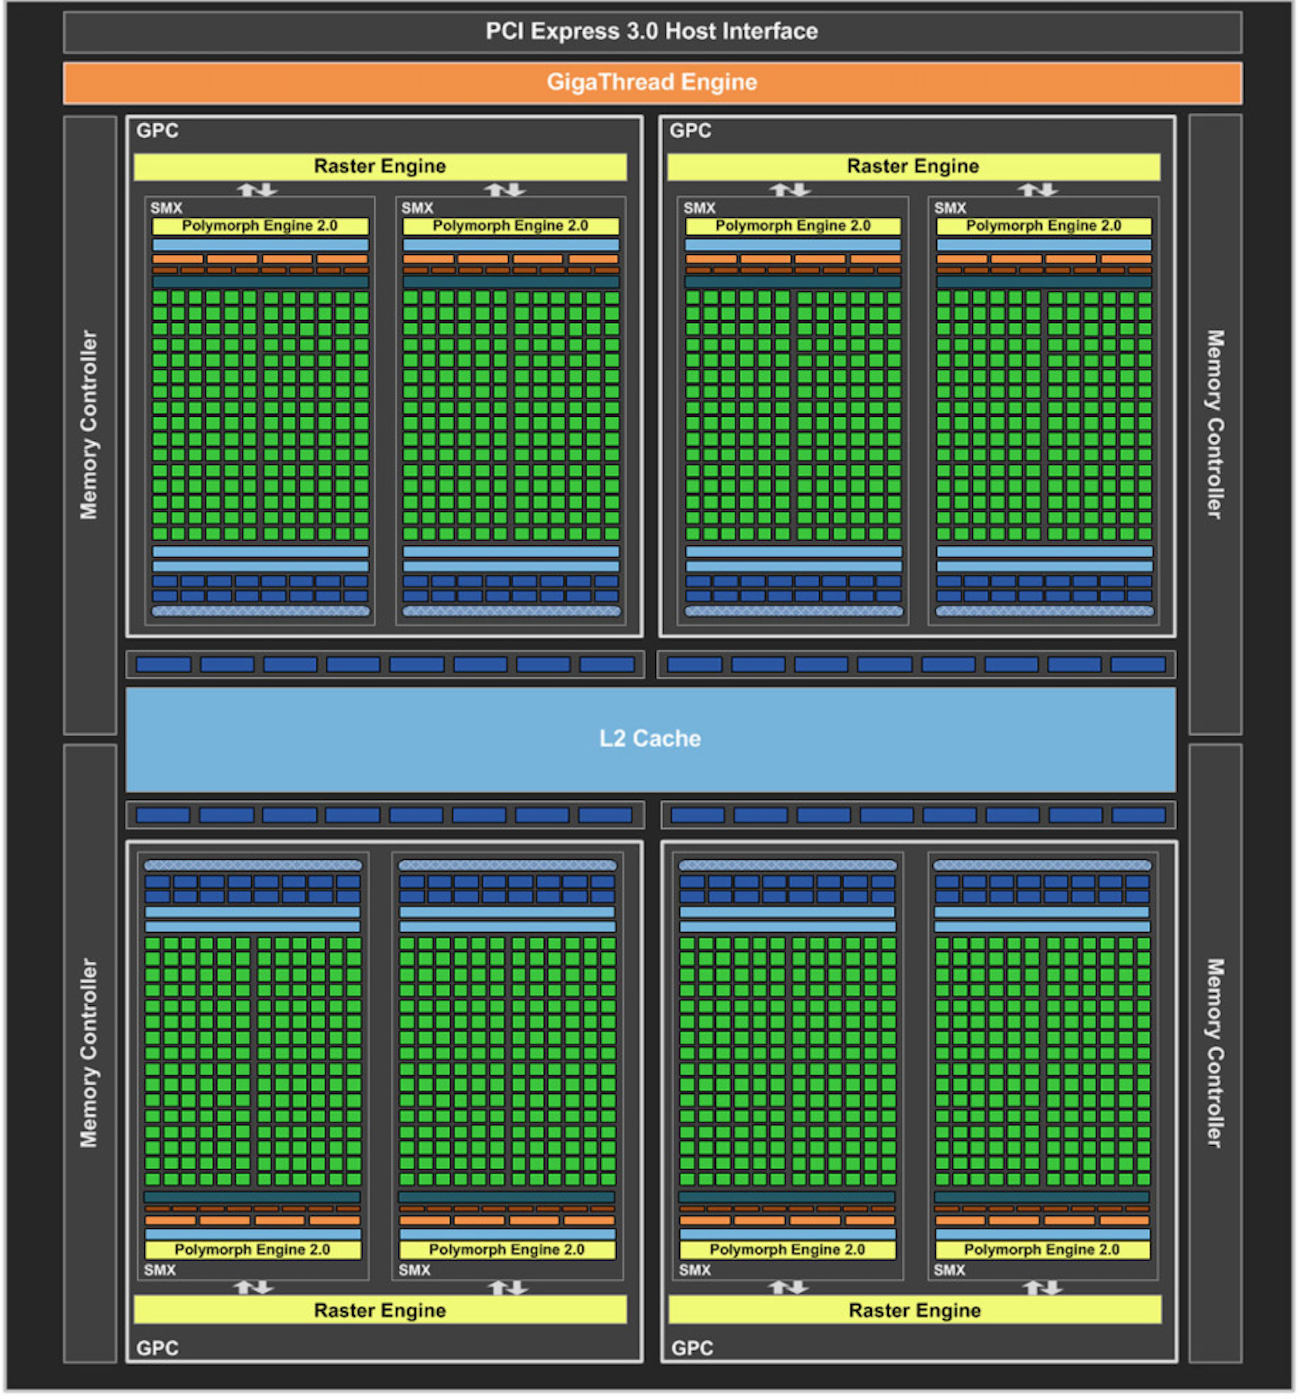
\includegraphics[scale=0.40]{Images/KeplerArch}
    \vspace{0.5in}
    \caption{Kepler Architecture.}
    \label{fig:KeplerArch}
\end{figure}

\begin{figure} [H]
    \centering
    \vspace{0.5in}
    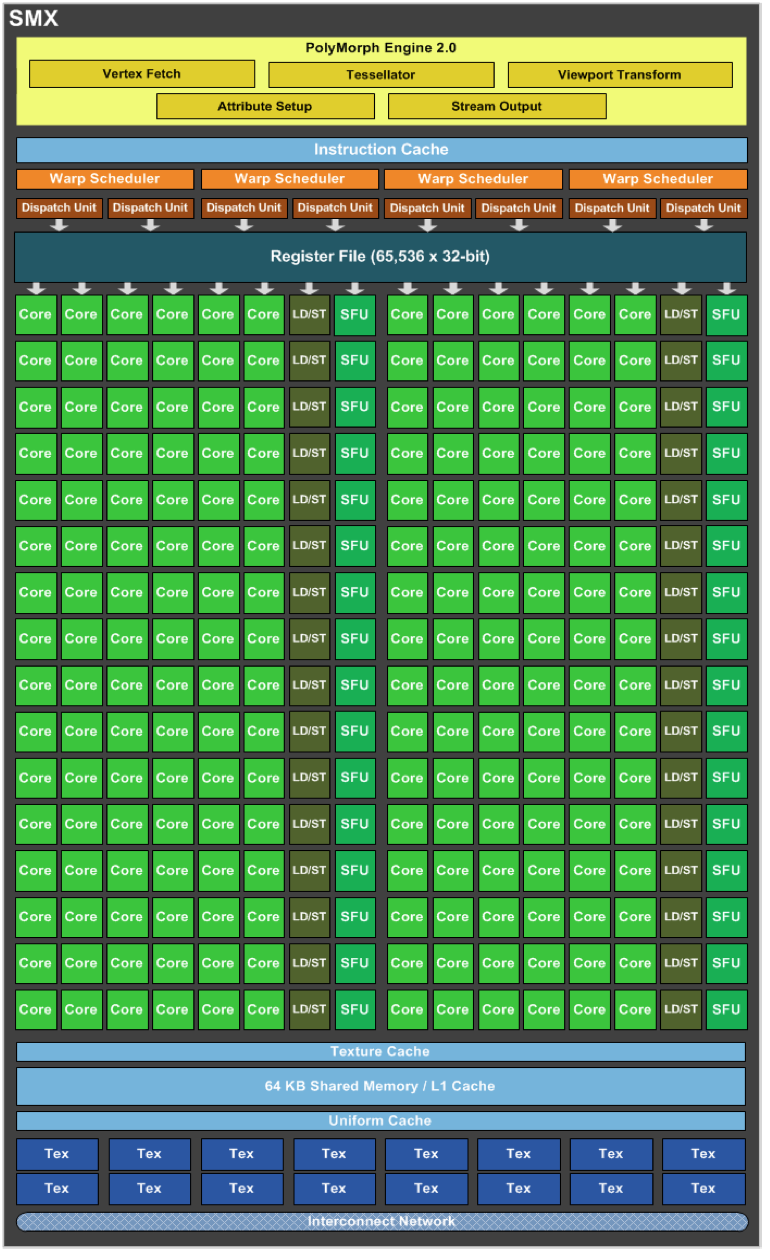
\includegraphics[scale=0.50]{Images/gpu_architecture}
    \vspace{0.5in}
    \caption{GTX680 SMX.}
    \label{fig:gpu_architecture}
\end{figure}

In Kepler, as shown in Figure~\ref{fig:memory}, each SMX has 64 KB of on-chip memory that can be configured as 48 KB of Shared memory with 16 KB of L1 cache, or as 16 KB of shared memory with 48 KB of L1 cache or a 32KB / 32KB split between shared memory and L1 cache.
In addition to the L1 cache, Kepler introduces a 48KB cache for data that is known to be read-only for the duration of the function and it also has a 1536KB of L2 cache memory.  The L2 cache services all loads, stores, and texture requests and provides high speed data sharing across the GPU~\cite{nvidia:12:gk110}.

\begin{figure} [H]
    \centering
    \vspace{0.5in}
    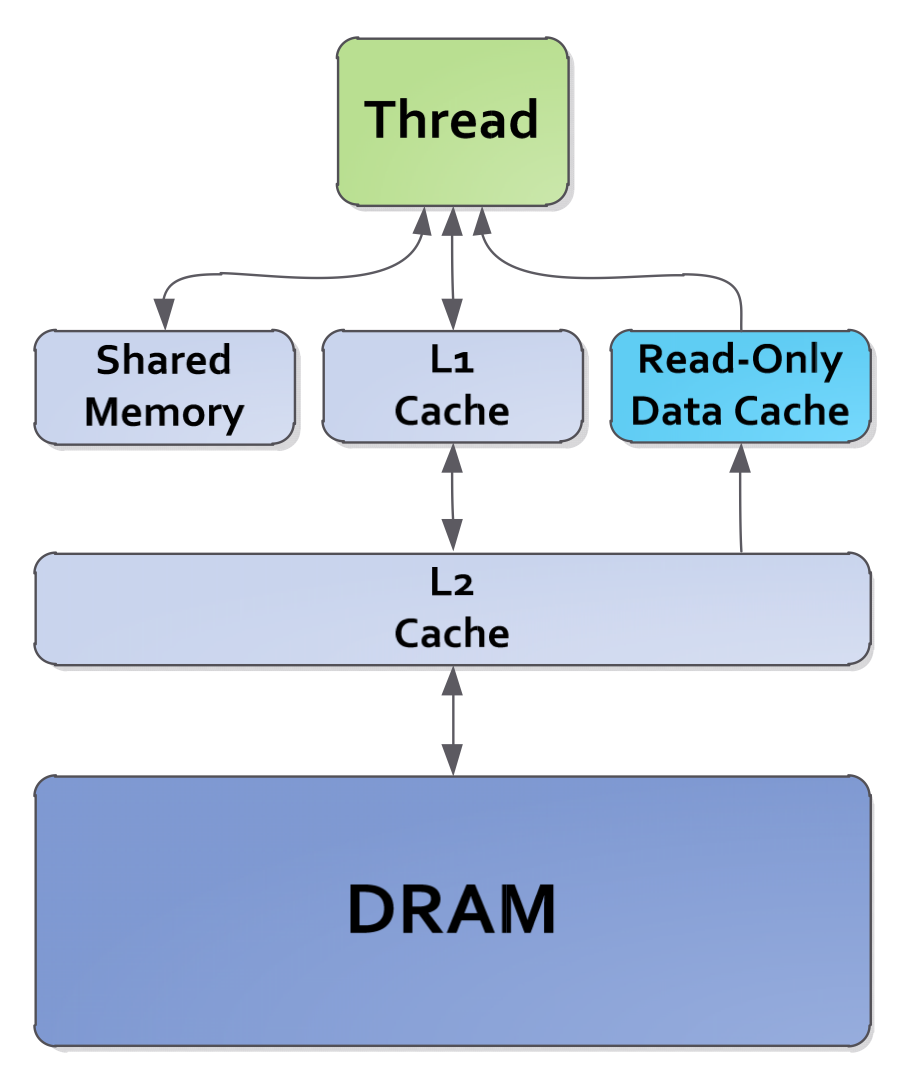
\includegraphics[scale=0.40]{Images/memory}
    \vspace{0.5in}
    \caption{Kepler Memory Hierarchy.}
    \label{fig:memory}
\end{figure}


%%%%%%%%%% GPU Interface (traditional vs CUDA)
%DAC:Must think in graphics terms to use
%    Restrictive programming models and instruction sets
%    Primitive tools Rapidly changing interfaces
Graphics processors have traditionally been designed for very specific
specialized tasks.  Most of their transistors perform calculations related
to 3D computer graphics rendering.  Typically GPUs perform memory-intensive
work such as texture mapping and rendering polygons.  The GPU also performs
geometric calculations such as rotation and translation of vertices into
different coordinate systems.  The on-chip programmable shaders can manipulate 
vertices and textures.  

NVIDIA\textsuperscript{\textregistered} has developed a parallel computing
architecture which is known as the Compute Unified Device Architecture (CUDA).  
This computing engine, which is the core of modern
NVIDIA\textsuperscript{\textregistered} GPUs, is accessible to software
developers through extensions of industry standard programming languages.  The
development of CUDA has enabled developers to access the virtual instruction
set and memory of the GPU. This has enabled the exploitation of the native
parallel computational elements of the NVIDIA\textsuperscript{\textregistered}
GPU. 

The Kepler architecture that has the Compute Capability 3.5 or higher supports dynamic parallelism, in which the GPU can launch new grids by itself. This feature allows algorithms that involve nested parallelism, recursive parallelism to be implemented on GPUs. This results in better GPU utilization than before. In Figure~\ref{fig:gpu_execution_hl_overview}, the Kepler host to GPU workflow 
shows the Grid Management Unit, which allows it to manage the actively 
dispatching grids, pause dispatch, and hold pending and suspended grids~\cite{nvidia:12:gk110}.

\begin{figure} [H]
    \centering
    \vspace{0.5in}
    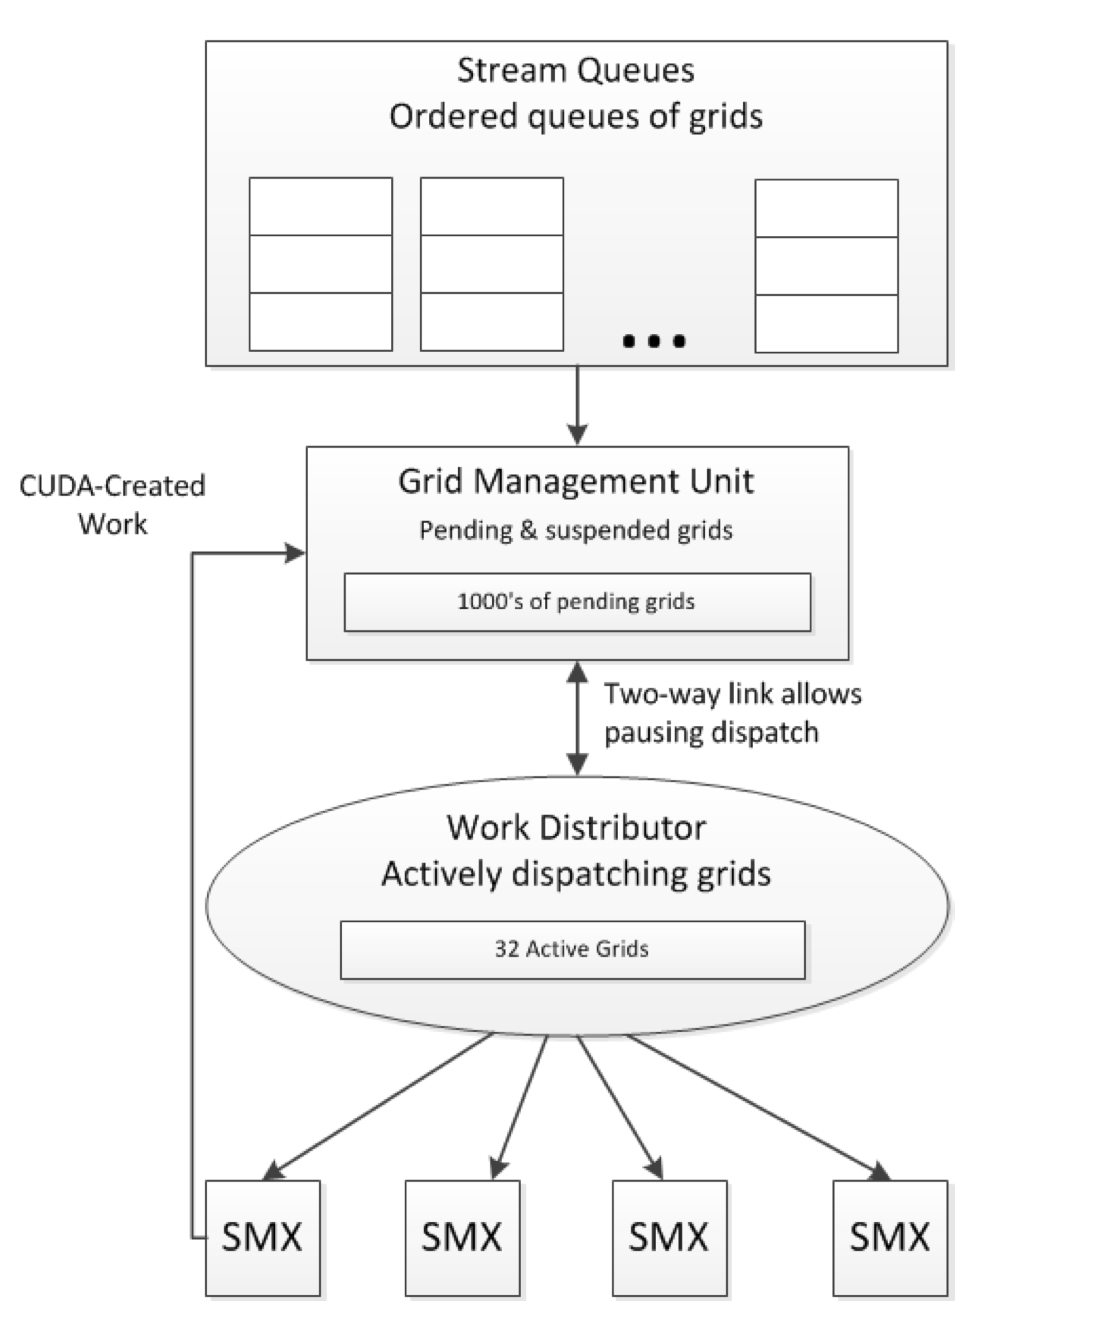
\includegraphics[scale=0.40]{Images/gpu_execution_hl_overview}
    \vspace{0.5in}
    \caption{Kepler Work Flow.}
    \label{fig:gpu_execution_hl_overview}
\end{figure}

%Scalablity and future compatibility

The CUDA model is optimized for maximum compatibility.
NVIDIA\textsuperscript{\textregistered} utilizes a soft instruction
set which enables the GPU designers to change the low level hardware
and instruction set without having to address backwards compatibility.
Similarly, NVIDIA\textsuperscript{\textregistered} has also built in
scalability to the CUDA model.  These GPUs are scalable in that the
CUDA code that is written is not tied to a specific release of the
NVIDIA\textsuperscript{\textregistered} GPU.  This can be contrasted
to traditional CPUs where the hard instruction set is published.  CPU
software developers often optimize their programs for how many cores
are available which can change as new CPUs are released.

A CUDA program
is comprised of multiple execution phases. Depending on the phase,
the execution involves the CPU, the GPU or both. Portions of the CUDA
code are executed on the GPU while other portions are executed on the
CPU.  The NVIDIA\textsuperscript{\textregistered} compiler known as
\textit{nvcc} translates the code for the GPU and CPU accordingly.
This model is very easy to work with because the device code is
written in ANSI C extended with keywords for labeling data-parallel
functions, called \textit{kernels}, and their associated data
structures~\cite{owens:08:gc}.

GPU implements a Single instruction multiple data (SIMD) model unlike the traditional CPU architectures where each thread may execute its own set of instructions. Multiple processing units are controlled by the same control signal from the control unit. Though each unit executes the same instruction, they have different data that corresponds to the CUDA threads.

 The GPU hardware maps the data blocks to the SMX through time and space multiplexing. Since each SMX has limited hardware resources such as shared memory, registers, number of threads that can be tracked and scheduled (scheduling lots), careful selection of block sizes allow the SMX to accommodate more blocks simultaneously thus increasing the throughput. 
 

%%%%%%%%%%%%%%%%%%%%%%%%%%%%%%%%%%%%%%%%%%%%%%%%%%%%%%%%%%%%%%%%%%%%%%%%%%%%%%%
\section{Motivation}~\label{sec:motivation}
%%%%%%%%%%%%%%%%%%%%%%%%%%%%%%%%%%%%%%%%%%%%%%%%%%%%%%%%%%%%%%%%%%%%%%%%%%%%%%%

In theory, for n items, the quadtree gives a performance of
${(n*log(n))}$. Compared to a brute force method's performance of
$n^{(2)}$~\cite{Eppstein:2000:FHC:351827.351829}, a quadtree is extremely fast. The performance gain by
using a quadtree is ${(log(n))/n}$.  As shown in
Figure~\ref{fig:comparing_bruteforce_cpu}, the empirical investigation
of quadtree search and brute force search shows that the quadtree has
a 9x better performance for medium number of queries and 8x
improvement for larger problems.  The main purpose of quadtree lies in
localizing the queries. The brute force search on a CPU checks
sequentially if every single point of the input data satisfies the
criteria whereas quadtrees help isolate the region of interest faster
by ignoring the quadrants of the tree that lie outside the region of
interest at every level, thus reducing the number of quadrants to be
processed at the next level. Therefore the quadtree gives better
performance for a dense more concentrated data than a dense equally
distributed data set.


\begin{figure}[H]
\centering
\vspace{0.5in}
    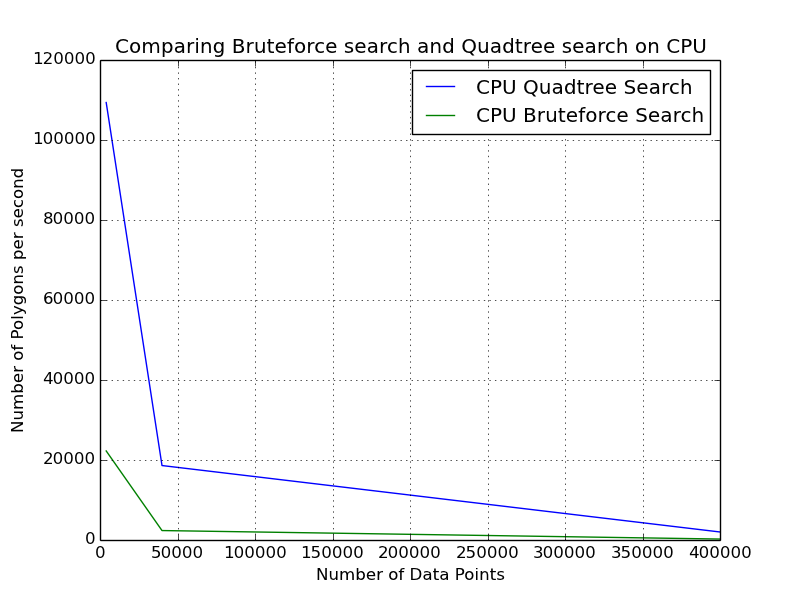
\includegraphics[scale=0.55]{Images/BruteVsQuadCPU_logscale_new_2}
    \vspace{0.5in}
    \caption{Comparing Bruteforce Search and Quadtree Search on CPU.}
    \label{fig:comparing_bruteforce_cpu}
  \end{figure}

As shown in Figure~\ref{fig:comparing_bruteforce_gpu}, the GPU provides a
better performance for brute force search compared to CPU for larger
datasets. But this performance is still lower than the CPU performance
using a quadtree. The same algorithm is used for both CPU and GPU
brute force search to check if a point is within the Polygon. But the
GPU is capable of launching 65535 blocks with a maximum of 1024
threads, thus massively parallelizing the search. The Geforce GTX680
Kepler architecture used, has a new parallel geometry pipeline
optimized for tessellation and displacement mapping. And also it has a
better performance / watt~\cite{nvidia:12:gtx680tech}.

\begin{figure}[H]
\centering
\vspace{0.5in}
    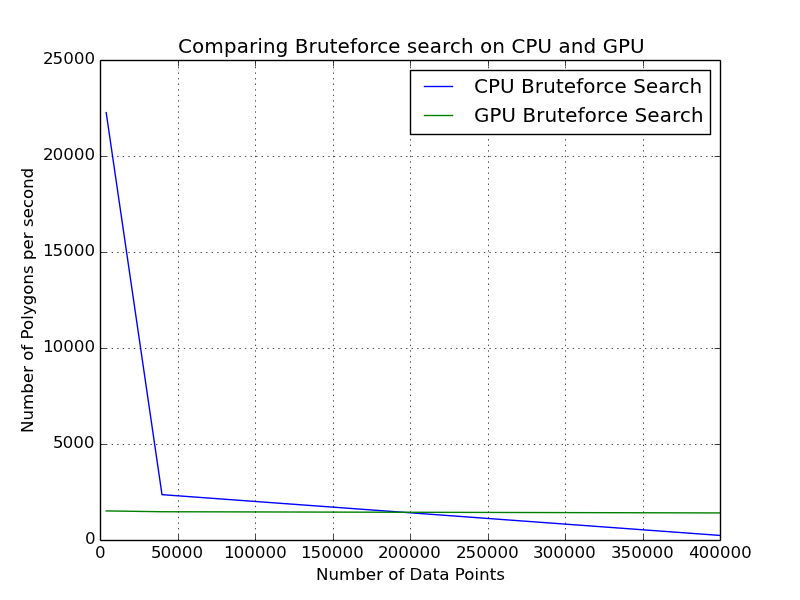
\includegraphics[scale=0.55]{Images/CPU_GPU_brute_new_2}
    \vspace{0.5in}
    \caption{Comparing Bruteforce Search on CPU with GPU.}
    \label{fig:comparing_bruteforce_gpu}
  \end{figure}

Figure~\ref{fig:cpu_quadtree_performance} shows the quadtree performance for different sized polygons. The small polygons occupy 10 to 20 percent of the quadtree area, the medium sized polygons occupy 30 to 60 percent of the quadtree area and the large polygons occupy 70 to 90 percent of the quadtree area.
The CPU implementation performs better on small polygons compared to larger polygons. The performance improvement in this case relates to how quickly the quadrants of the quadtree that contain the polygon can be isolated. The amount of computation done for a larger polygon that occupies all four quadrants is higher compared to a smaller polygon that lies inside only one quadrant.

\begin{figure}[H]
\centering
\vspace{0.5in}
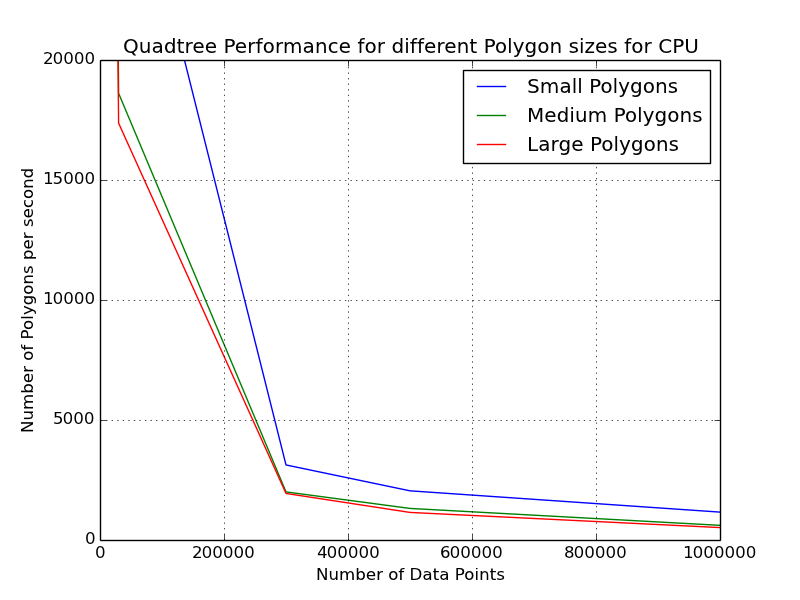
\includegraphics[scale=0.55]{Images/Different_Sized_Polygon_logScale_cpu04_10}
\vspace{0.5in}
\caption{CPU Performance of Different Sized Polygons using Quadtree.}
\label{fig:cpu_quadtree_performance}
\end{figure}

